%!TEX TS-program = xelatex
%!TEX encoding = UTF-8 Unicode

\documentclass[11pt,tikz,border=1]{standalone}
\usepackage{pgfplots}
\usetikzlibrary{positioning}

\begin{document}
  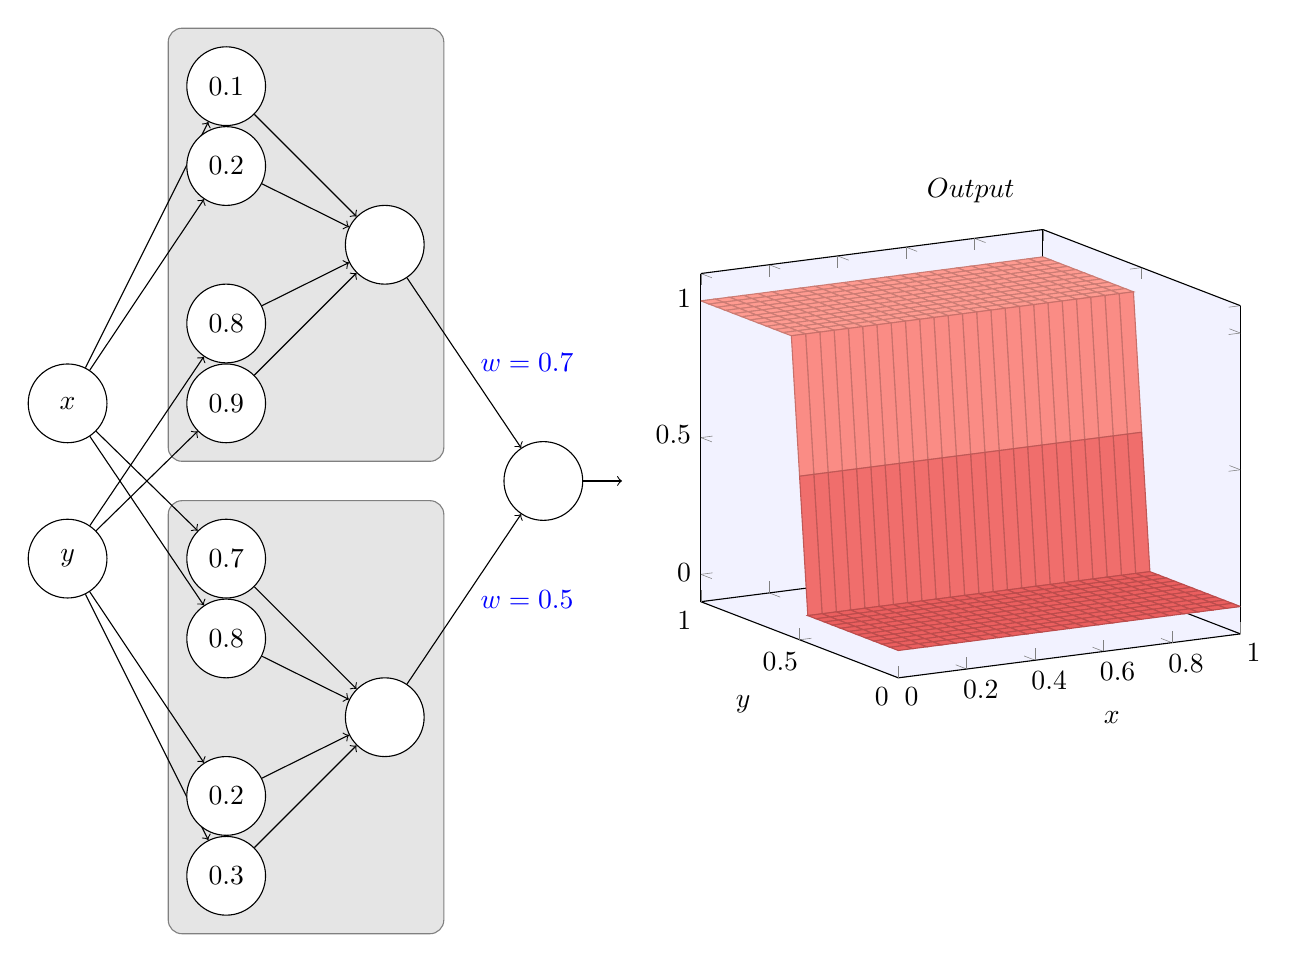
\begin{tikzpicture}[
    neuron/.style={circle,draw,fill=white,inner sep=0pt,minimum size=10mm},
    invisible/.style={circle,inner sep=0pt,minimum size=10mm},
    box/.style={rectangle,draw=gray,fill=gray!20,rounded corners=5pt,minimum width=3.5cm,minimum height=5.5cm}
    ]
    
    \begin{scope}
      \node(output) [neuron] {};

      \node(box0) [box,left=of output,xshift=2.5mm,yshift=3cm] {};
      \node(box1) [box,left=of output,xshift=2.5mm,yshift=-3cm] {};
      
      \node(box0output) [neuron,left=of output,yshift=3cm] {};
      \node(box0s1) [invisible,left=of box0output,yshift=1cm] {};
      \node(box0s2) [neuron,left=of box0output,yshift=-1cm] {$0.8$};
      \node(box0s0) [neuron,above] at (box0s1.north) {$0.1$};
      \node(box0s3) [neuron,below] at (box0s2.south) {$0.9$};

      \node(box1output) [neuron,left=of output,yshift=-3cm] {};
      \node(box1s1) [neuron,left=of box1output,yshift=1cm] {$0.8$};
      \node(box1s2) [invisible,left=of box1output,yshift=-1cm] {};
      \node(box1s0) [neuron,above] at (box1s1.north) {$0.7$};
      \node(box1s3) [neuron,below] at (box1s2.south) {$0.3$};

      \node(x) [neuron,left=of box0s3] {$x$};
      \node(y) [neuron,left=of box1s0] {$y$};
      
      \foreach \x in {0,...,3} {
        \draw[->] (box0s\x) to (box0output);
        \draw[->] (box1s\x) to (box1output);
      }
      
      \draw[->] (x) to (box0s0);
      \draw[->] (x) to (box0s1);
      \draw[->] (x) to (box1s0);
      \draw[->] (x) to (box1s1);
      \draw[->] (y) to (box0s2);
      \draw[->] (y) to (box0s3);
      \draw[->] (y) to (box1s2);
      \draw[->] (y) to (box1s3);
      
      \node(box0s1a) [neuron] at (box0s1.center) {$0.2$};
      \node(box1s2a) [neuron] at (box1s2.center) {$0.2$};

      \draw[->] (box0output) -- node [blue,xshift=8mm] {$w = 0.7$} (output);
      \draw[->] (box1output) -- node [blue,xshift=8mm] {$w = 0.5$} (output);

      \draw[->] (output) -- ++(1cm, 0);
    \end{scope}
    
    \begin{scope}[xshift=2cm,yshift=-2.5cm]    
      % FIXME: rotate the zlabel, change plot color, and move z axis to right
      \begin{axis}[
        view={-30}{15},        
        axis background/.style={fill=blue!5},
        xlabel=$x$,
        ylabel=$y$,
        title=$Output$,
        colormap={simple}{rgb255=(235,95,95) rgb255=(255,155,145)},
        declare function={
          sigmaInverse(\z)=ln(\z/(1-\z));
          f(\x)=0.2+0.4*\x*\x+0.3*\x*sin(15*deg(\x))+0.05*cos(50*deg(\x));
        }]
        \addplot3[surf,domain=0:1] {
          1 / (1 + exp(-(1000) * y - (-0.5 * 1000)))
        };
      \end{axis}
    \end{scope}
    
  \end{tikzpicture} 
\end{document}
